\documentclass{source/Report}

\major{地理信息科学}
\name{陈杰伟}
\title{RV64 虚拟内存}
\stuid{3200101205}
\college{地球科学学院}
\date{\today}
\lab{玉泉曹光彪-西503}
\course{操作系统}
\instructor{寿黎但}
\grades{}
\expname{RV64 虚拟内存}
\exptype{编程实验}
\partner{无}

\begin{document}
\makecover
\makeheader
\section{实验目的}

- 学习虚拟内存的相关知识,实现物理地址到虚拟地址的切换。

- 了解 RISC-V 架构中 SV39 分页模式,实现虚拟地址到物理地址的映射,并对不同的段进行相应的权限设置。

\section{实验环境}
Ubuntu 20.04

\section{实验步骤}
\subsection{setup\_vm的实现}

将 0x80000000 开始的 1GB 区域进行两次映射,其中一次是等值映射 ( PA == VA ) ,另一次是将其映射至高地址 ( PA + PV2VA\_OFFSET == VA )。
OS run 起来的时候, 其本身就是一个线程 idle线程, 第一步为 idle 设置 task\_struct。并将 current, task[0] 都指向 idle。


\begin{lstlisting}[language = c, title = {setup\_vm}]
void setup_vm(void)
{

    /*  将 va 的 64bit 作为如下划分: | high bit | 9 bit | 30 bit |
        high bit 可以忽略
        中间9 bit 作为 early_pgtbl 的 index
        低 30 bit 作为 页内偏移 这里注意到 30 = 9 + 9 + 12, 即我们只使用根页表, 根页表的每个 entry 都对应 1GB 的区域。
    */
    // Page Table Entry 的权限 V | R | W | X 位设置为 1

    //注意:所有符号都被定义在虚拟地址,所以在启动虚拟地址需要反计算到物理地址(unsigned long *)((uint64)early_pgtbl - PA2VA_OFFSET)
    PHY_EARLY_PGTBL[((uint64)PHY_START << 25) >> 55] = (((uint64)PHY_START >> 30) << 28) + 0b0000001111; //等值映射

    PHY_EARLY_PGTBL[((uint64)VM_START << 25) >> 55] = (((uint64)PHY_START >> 30) << 28) + 0b0000001111; //至高映射

    return;
}
\end{lstlisting}

完成上述映射之后,通过 relocate 函数,完成对 satp 的设置,以及跳转到对应的虚拟地址。

\begin{lstlisting}[language = bash, title = {relocate}]
    relocate:
    # set ra = ra + PA2VA_OFFSET
    # set sp = sp + PA2VA_OFFSET (If you have set the sp before)

    li t0, PA2VA_OFFSET
    add ra, ra, t0
    add sp, sp, t0

    # set satp with early_pgtbl

    li t0, 0x8000000000000000
    la t1, early_pgtbl
    li t2, PA2VA_OFFSET
    sub t1, t1, t2
    srl t1, t1, 12
    add t0, t0, t1

    csrw satp, t0

    # flush tlb
    sfence.vma zero, zero

    # flush icache
    fence.i

    ret
\end{lstlisting}


\subsection{setup\_vm\_final 的实现}

由于 setup\_vm\_final 中需要申请页面的接口, 应该在其之前完成内存管理初始化, 可能需要修改 mm.c 中的代码,mm.c 中初始化的函数接收的起始结束地址需要调整为虚拟地址。

\begin{lstlisting}[language = c, title = {mm\_init}]
    void mm_init(void) {
        kfreerange(_ekernel, (char *)VM_KERNEL_END);
        printk("\n...mm_init done!\n");
    }
\end{lstlisting}

采用三级页表映射。    

\begin{lstlisting}[language = c, title = {setup\_vm\_final}]
    void setup_vm_final(void)
    {
        memset(swapper_pg_dir, 0x0, PGSIZE);
    
        // mapping kernel text X|-|R|V
        create_mapping(swapper_pg_dir, (uint64)_stext, PHY_ADR((uint64)_stext), (uint64)_etext - (uint64)_stext, (uint64)0b0000001011);
    
        // mapping kernel rodata -|-|R|V
        create_mapping(swapper_pg_dir, (uint64)_srodata, PHY_ADR((uint64)_srodata), (uint64)_erodata - (uint64)_srodata, (uint64)0b0000000011);
    
        // mapping other memory -|W|R|V
        create_mapping(swapper_pg_dir, (uint64)_sdata, PHY_ADR((uint64)_sdata), (uint64)VM_KERNEL_END - (uint64)_sdata, (uint64)0b0000000111);
    
        csr_write(satp, (uint64)(0x8000000000000000 + ((uint64)PHY_ADR(swapper_pg_dir) >> 12)));
    
        // flush TLB
        asm volatile("sfence.vma zero, zero");
    
        // flush icache
        asm volatile("fence.i");
    
        return;
    }
    
    /* 创建多级页表映射关系 */
    void create_mapping(uint64 *pgtbl, uint64 va, uint64 pa, uint64 sz, uint64 perm)
    {
        /*
        pgtbl 为根页表的基地址
        va, pa 为需要映射的虚拟地址、物理地址
        sz 为映射的大小
        perm 为映射的读写权限
    
        创建多级页表的时候使用 kalloc() 来获取一页作为页表目录
        使用 V bit 来判断页表项是否存在
        */
        uint64 offset = 0;
    
        // 0级页表4kb映射
        for (; offset < sz; offset += PGSIZE)
        {
            uint64 va_offset = va + offset;
    
            //获取vpn
            uint64 vpn[3] = {
                (va_offset << 43) >> 55,
                (va_offset << 34) >> 55,
                (va_offset << 25) >> 55};
    
            uint64 *pg_dir_l1 ,*pg_dir_l0;
    
            //1gb映射
            if (pgtbl[vpn[2]] == 0)
            {
                pg_dir_l1 = (uint64 *)kalloc();
                pgtbl[vpn[2]] = (((uint64)PHY_ADR(pg_dir_l1) >> 12) << 10) + NOT_LEAF_PERM;
            }
            else
                pg_dir_l1 = (uint64 *)(VIS_ADR((pgtbl[vpn[2]] >> 10) << 12));
    
            if (pg_dir_l1[vpn[1]] == 0)
            {
                pg_dir_l0 = (uint64 *)kalloc();
                pg_dir_l1[vpn[1]] = (((uint64)PHY_ADR(pg_dir_l0) >> 12) << 10) + NOT_LEAF_PERM;
            }
            else
                pg_dir_l0 = (uint64 *)(VIS_ADR((pg_dir_l1[vpn[1]] >> 10) << 12));
    
            pg_dir_l0[vpn[0]] = (uint64)((((pa + offset) >> 12) << 10) + perm);
        }
    
        return;
    }
\end{lstlisting}

在 head.S 中 适当的位置调用 setup\_vm\_final 。  

\begin{lstlisting}[language = bash, title = {head.S调用}]
    la sp, boot_stack_top #将栈指针寄存器指向栈顶地址

    call mm_init
    call setup_vm_final

    call task_init
\end{lstlisting}



\section{运行结果}

各个线程正确运行在其虚拟页上,如图一

\begin{figure}[p]
    \centering
    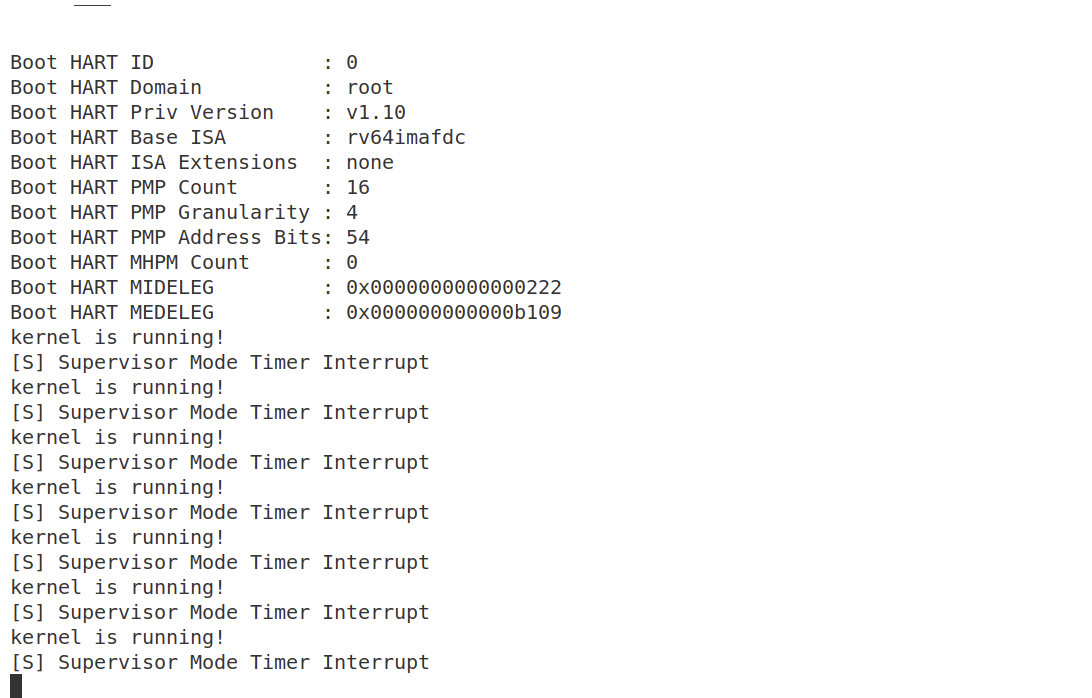
\includegraphics[width = 1\textwidth]{1}
    \caption{虚拟内存结果}
\end{figure}

\section{思考题}

1.验证 .text, .rodata 段的属性是否成功设置,给出截图。

对.text段,程序可运行在高地址的.text段,则其可执行

在dummy中调用如下代码

\begin{lstlisting}[language = c, title = {测试代码}]
    printk("%d", *((uint64 *)_stext)); // read text
    *((uint64 *)_stext) = 1; // write text
    printk("%d", *((uint64 *)_stext));
\end{lstlisting}

并在上述行和\_traps处打断点,开启调试

图2显示可以打印出\_stext内存存储值,证明可读

\begin{figure}[p]
    \centering
    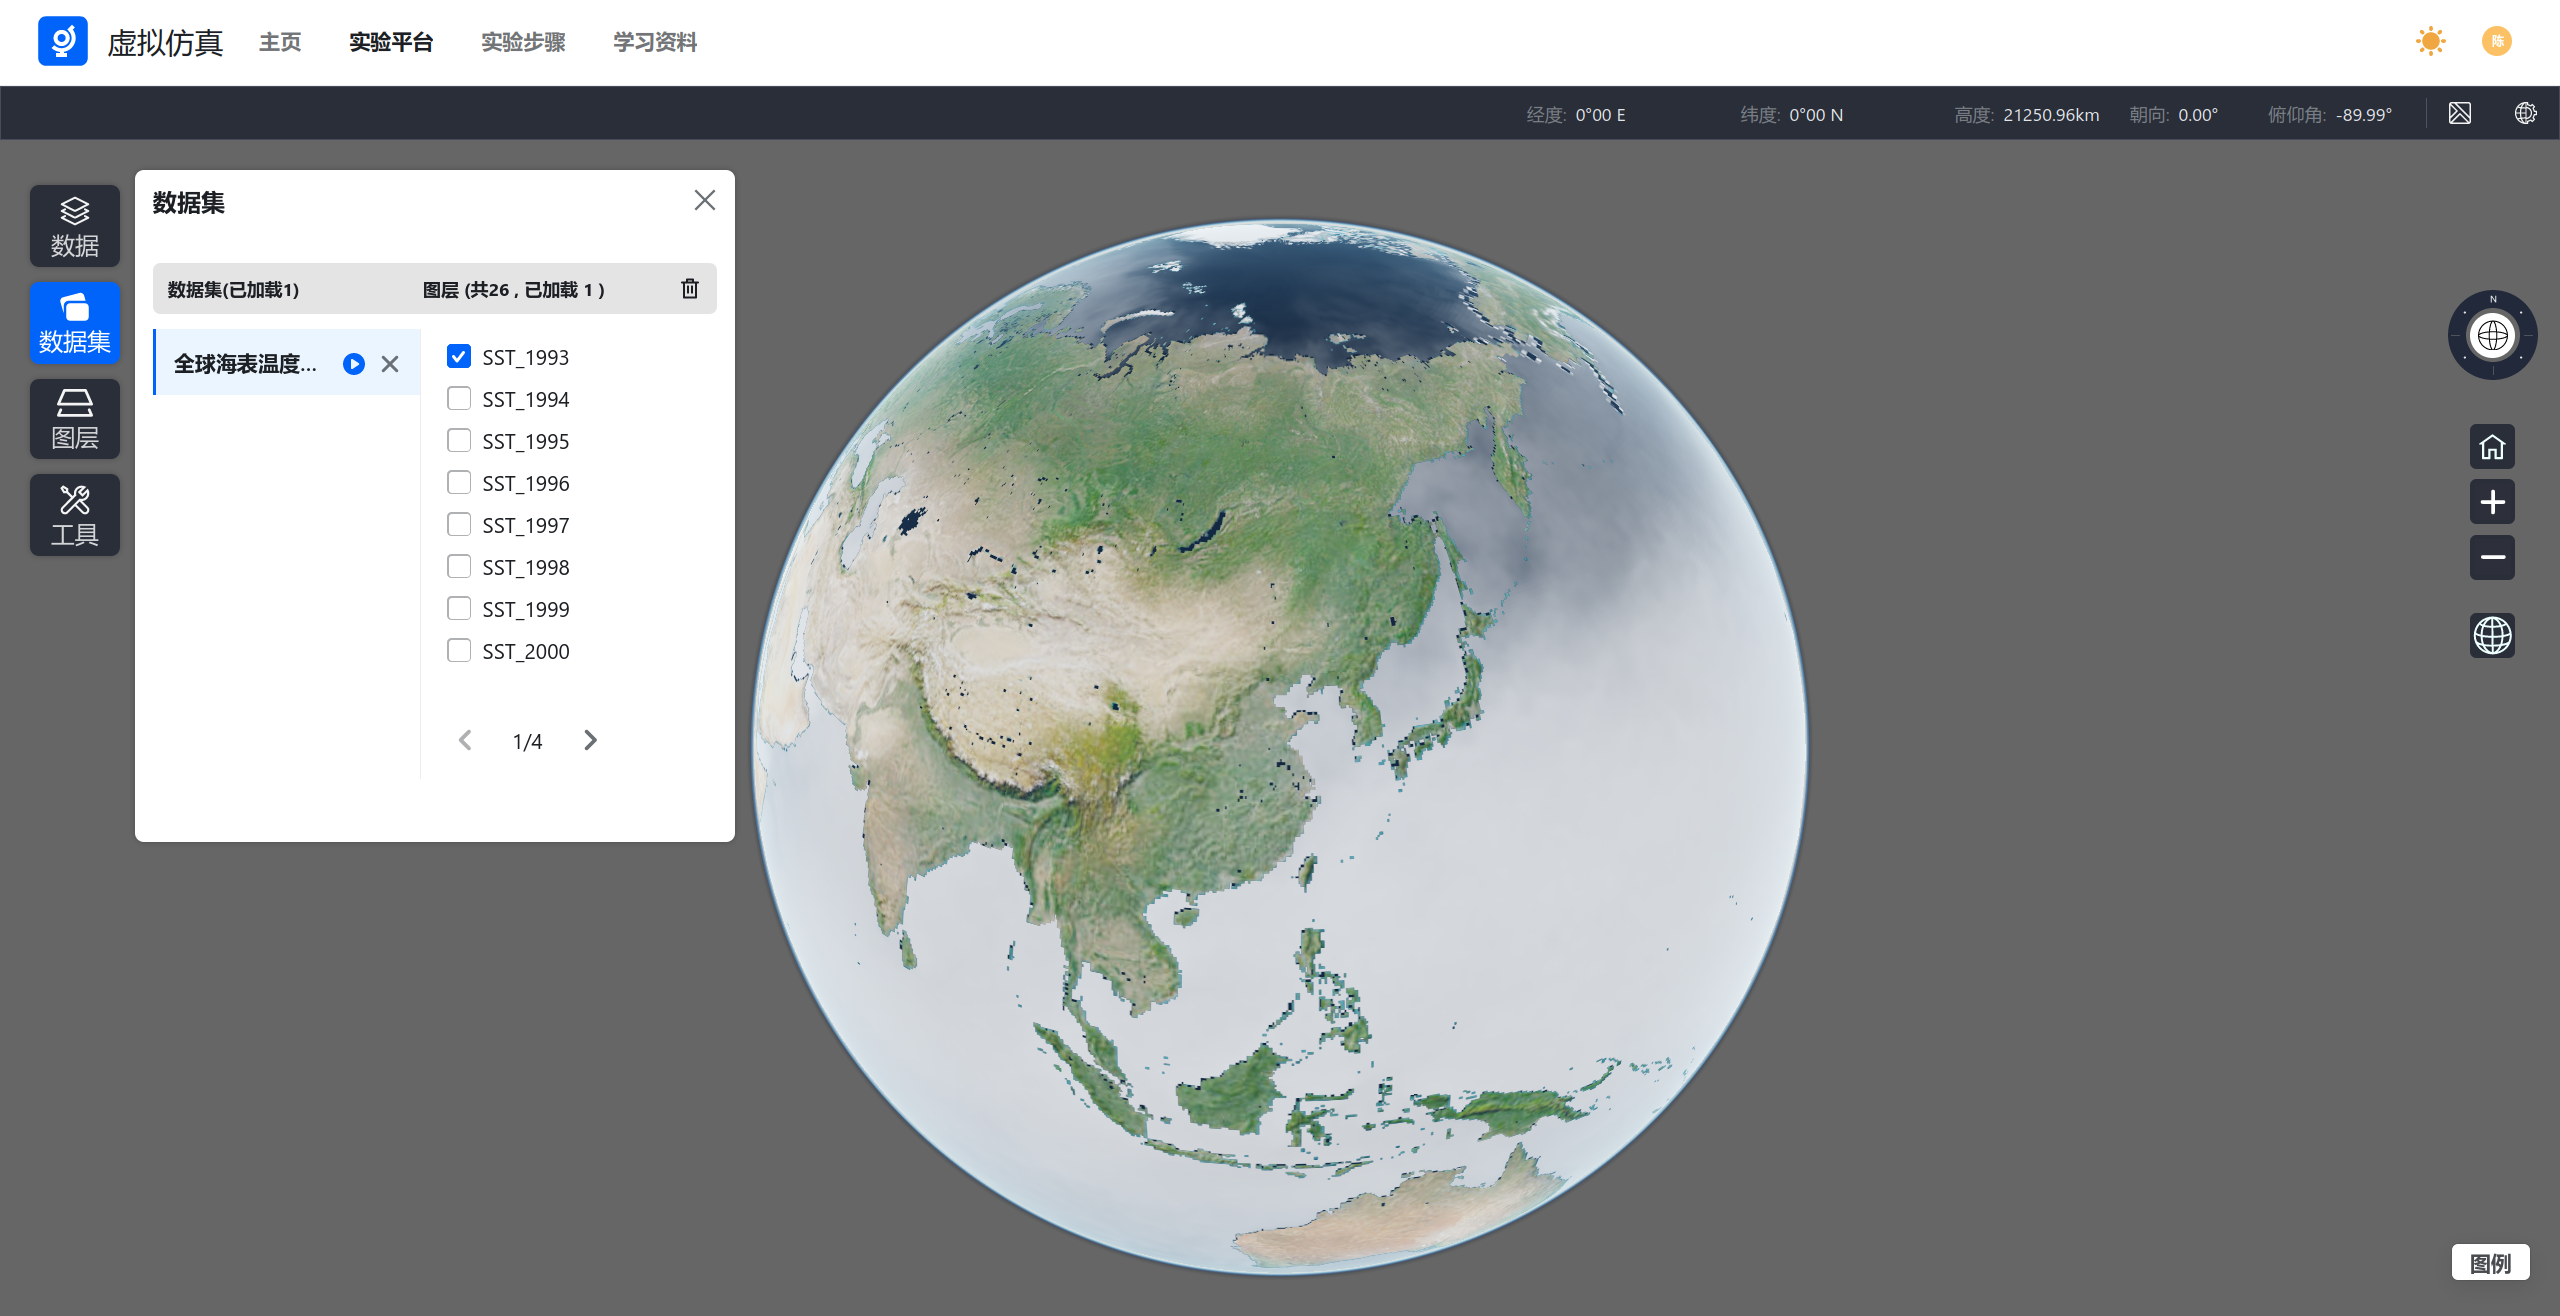
\includegraphics[width = 1\textwidth]{2}
    \caption{\_stext可读}
\end{figure}

图3显示向\_stext地址写入触发了中断,中断原因是store page fault证明该页不可写

\begin{figure}[p]
    \centering
    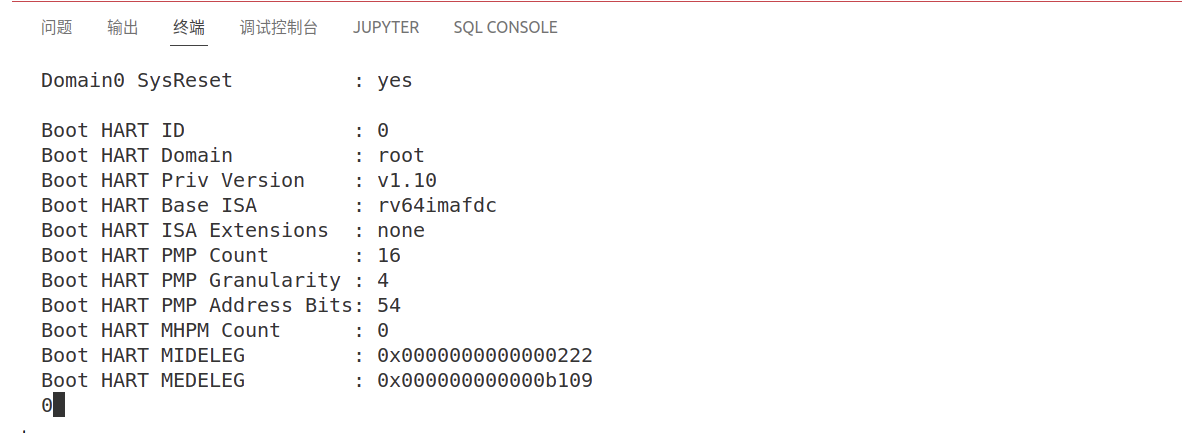
\includegraphics[width = 1\textwidth]{3}
    \caption{\_stext不可写}
\end{figure}

同样的对于.rodata段

\begin{lstlisting}[language = c, title = {测试代码}]
    printk("%d", *((uint64 *)_srodata)); // read text
    *((uint64 *)_srodata) = 1; // write text
    printk("%d", *((uint64 *)_srodata));
\end{lstlisting}

图4显示可以打印出\_srodata内存存储值,证明可读

\begin{figure}[p]
    \centering
    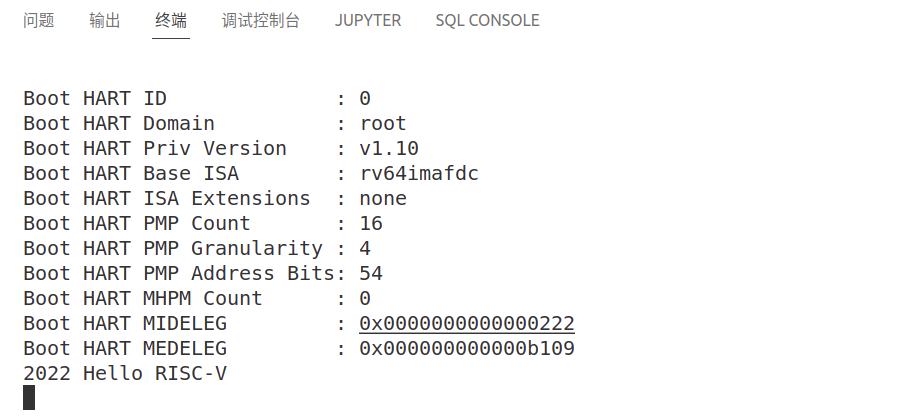
\includegraphics[width = 1\textwidth]{4}
    \caption{\_srodata可读}
\end{figure}

图5显示向\_srodata地址写入触发了中断,中断原因是store page fault证明该页不可写

\begin{figure}[p]
    \centering
    
\includegraphics[width = 1\textwidth]{5}
    \caption{\_srodata不可写}
\end{figure}

2. 为什么我们在 setup\_vm 中需要做等值映射?

因为在写入satp开启虚拟内存后我们还需要做一系列操作和跳转至虚拟内存,而此时PC寄存器仍然指在物理地址上所以要对物理地址做等值映射才能确保程序继续执行

3. 在 Linux 中,是不需要做等值映射的。请探索一下不在 setup\_vm 中做等值映射的方法。

Linux采用懒加载策略(lazy allocation)在读到虚拟内存产生page fault后,系统从一个结构vm\_area中读取到虚拟内存定义的范围,如果范围显示该虚拟内存合法,则在此时做虚拟内存映射,否则抛出page fault

\end{document}

